% !TEX root = ../../article.tex

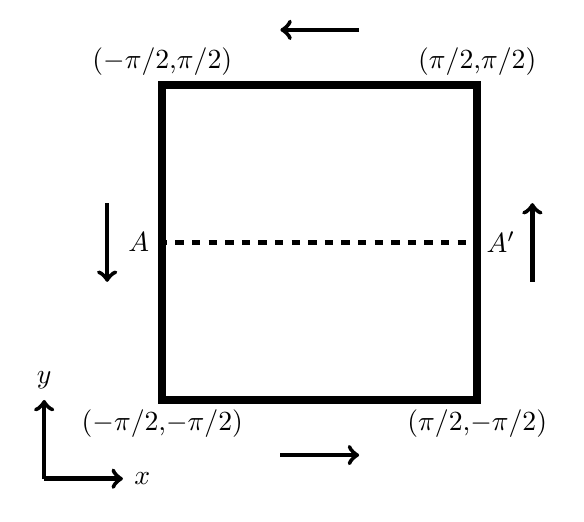
\begin{tikzpicture}
	\draw[line width=1mm] (-2,-2) rectangle (2,2);
    % axes
	\draw[->,ultra thick] (-3.5,-3)--(-2.5,-3) node[right]{$x$};
	\draw[->,ultra thick] (-3.5,-3)--(-3.5,-2) node[above]{$y$};
    % notable points
    \node[] at (-2,-2.3) (bl_corner) {($-\pi/2$,$-\pi/2$)};
    \node[] at (2,-2.3) (br_corner) {($\pi/2$,$-\pi/2$)};
    \node[] at (-2,2.3) (tl_corner) {($-\pi/2$,$\pi/2$)};
    \node[] at (2,2.3) (tr_corner) {($\pi/2$,$\pi/2$)};
	% lines AA' and BB'
	\node[] at (-2.3,0) (a) {$A$};
	\node[] at (2.3,0) (b) {$A'$};
	\draw[dashed,ultra thick] (a.east)--(b);
	% \node[] at (0,-2.3) (c) {$B$};
	% \node[] at (0,2.3) (d) {$B'$};
	% \draw[dashed,ultra thick] (c)--(d);
	% boundary velocity arrows
	\draw[->,ultra thick] (0.5,2.7)--(-0.5,2.7); %top
    \draw[->,ultra thick] (-0.5,-2.7)--(0.5,-2.7); %bottom
    \draw[->,ultra thick] (-2.7,0.5)--(-2.7,-0.5); %left
    \draw[->,ultra thick] (2.7,-0.5)--(2.7,0.5); %right
\end{tikzpicture}
